\section{सर्किट डिज़ाइन}
	\begin{figure}[ht!]
	\begin{tikzpicture}
		[->,>=stealth',semithick]	
		\node[rectangle,draw] (r0) at (0, 0) {फोटोडायोड};
		\node[rectangle,draw,text width=1cm, align=center] (r1) at (-1, -2) {लाल LED};
		\node[rectangle,draw,text width=1cm, align=center] (r2) at (1, -2) {इन्फ़्रारेड LED};	
		\node[rectangle,draw,text width=1cm, align=center] (r3) at (0, -4) {LED चालक};
		\node[rectangle,draw,text width=3cm, align=center] (r4) at (4, 0) {ट्रांस्इम्पेडेंस एम्पलीफायर};
		\node[rectangle,draw,text width=2cm, align=center]  (r5) at (8, 0) {डिफ़ैंस एम्पलीफायर};
		\node[rectangle,draw,text width=2cm, align=center] (r6) at (8, -2) {प्रोग्रामेबल गेन एम्प्लिफायर};
		\node[rectangle,draw,text width=3cm, align=center] (r7) at (8, -4) {$\mu$C ADC};
		\node[rectangle,draw,text width=1cm, align=center] (r8) at (2, -4) {$\mu$C};
		\node[rectangle,draw,text width=1cm, align=center] (r9) at (5, -2) {$\mu$C};
		
		\path (r1) edge (r0);
		\path (r2) edge (r0);
		\path (r3) edge (r1) 
		edge (r2);
		\path (r0) edge (r4);
		\path (r4) edge (r5);
		\path (r5) edge (r6);
		\path (r6) edge (r7);
		\path (r8) edge (r3);
		\path (r9) edge (r6);
		
	\end{tikzpicture}
	\caption{सिस्टम ब्लॉक आकृति}
	\end{figure}

	ब्लॉक आकृति का जिक्र करते हुए, उपखंड नीचे विभाजित हैं जो सर्किट और संबंधित आसिलोस्कोप ट्रेस आउटपुट दिखाते हैं।
	
	\subsection{फ्रंट एंड}	
	
		\subsubsection{ट्रांस्इम्पेडेंस भाग}
		
			फोटोडायोड के करंट को आनुपातिक वोल्टेज में बदलने की आवश्यकता होती है ताकि अंततः माइक्रोकंट्रोलर SpO\textsubscript{2} की गणना के लिए ADC का उपयोग करके वोल्टेज को डिजिटल मान में परिवर्तित कर सके। इसे प्राप्त करने के लिए एक साधारण ट्रांजिम्पेडेंस एम्प्लीफायर कॉन्फ़िगरेशन का उपयोग किया गया हैं:
			
			
			\begin{figure}[ht!]\centering
				\begin{circuitikz}[american] 
					\draw
					
					(2,3) node[op amp,yscale=-1] (opamp) {}
					(opamp.down) -- +(0,0.3) node[vcc]{Vcc}
					(opamp.up) -- +(0,-0.3) node[ground]{}
					(0,0) node[ground]{} to[pDo, l^=$D$, f^=$I$]  (0,2.5) to (opamp.-)
					(opamp.+) node[ground]{}
					(opamp.-) -- ++(0,-1.7) -- ++(0.5,0)
					to [R, l^=$R_1$] ++(1.5,0) -- ++(0.4,0) to (opamp.out)
					(opamp.-)  ++(0,-1.7) -- ++(0,-1.3) -- ++(0.5,0) 
					to [C, l^=$C_1$]  ++(1.5,0) -- ++(0.4,0) -- ++(0,1.3) 
					(opamp.out) -- ++(1,0) to [open,v=$V_1$,o-o] ++(0,-3) node[ground]{};
					
				\end{circuitikz}
			\end{figure}
			
		
			Led की तीव्रता के अनुसार, यदि फोटोडायोड में 10$\mu$A का करंट उत्पन्न होता है, और R = 100K$\Omega$, ओम के नियम के अनुसार, $V_1$ = 1 V। 
			कैपेसिटर का उपयोग पल्स कि लो-पास फ़िल्टरिंग के लिए किया जाता है। कट ऑफ आवृत्ति होगी:
		
			\begin{equation}	
				F_c = \frac{1}{2\pi R_1C_1}
			\end{equation}
			
			यदि R\textsubscript{1}=576K$\Omega$, C\textsubscript{1} = 33pF, 

			\[	
			F_c \approx \SI{8.3}{\kilo\hertz}
			\]
			
			\begin{figure}[ht!]
				\centering
				\subfloat[V\textsubscript{1} 
				]{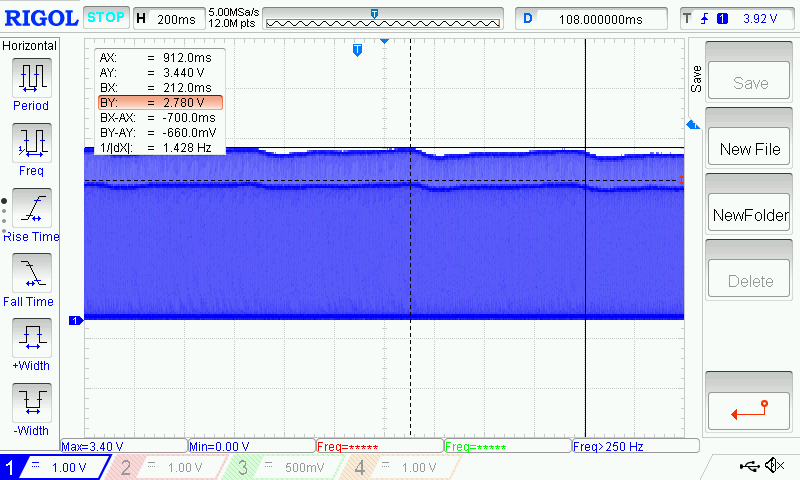
\includegraphics[width=0.9\textwidth]{../common/circuit/itov.png}}
				\hfill
				\subfloat[V\textsubscript{1} ज़ूम 
				]{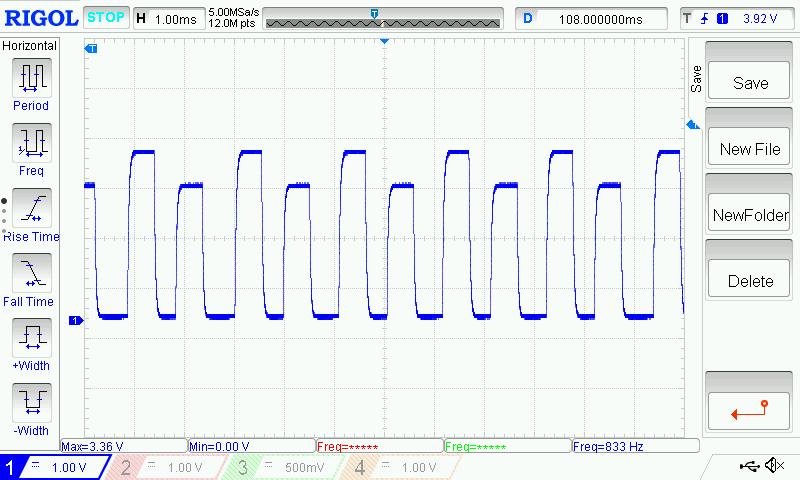
\includegraphics[width=0.9\textwidth]{../common/circuit/itov_zoom.png}
				\label{fig:itov}}
				\caption{V\textsubscript{1} ऑसिलोस्कोप ट्रेस (लाल \& इन्फ़्रारेड क्रमिक रूप से स्पंदित) }
			\end{figure}
			
			चूंकि led क्रमिक रूप से तेज दर के साथ ऑन-ऑफ होते हैं, इसलिए पल्स एक वर्ग तरंग की तरह दिखाई देगा। हमें led को स्पंदित करने के लिए इस कट-ऑफ के 1/10\textsuperscript{th} से कम पल्स फ्रीक्वेंसी का उपयोग करने होगा ताकि इसके सभी उच्च-आवृत्ति घटकों के साथ वर्ग तरंग स्पष्ट रूप से दिखाई दे और फ़िल्टर न हो।
			
			\[	
			F_p = \SI{500}{\hertz}
			\]
					
			
			यह ट्रेस में देखा जा सकता है, डीसी स्तर के उपर 2 PPG सिग्नल मोजुद हैं।
			उच्च आयाम इन्फ़्ररेड स्पंदन का परिणाम है, जबकि निचला आयाम लाल का है। चूँकि चोटियाँ हृदय गति के अनुरूप होती हैं, ट्रेस अनुसार यह 1.42/सेकंड या 85BPM है। सिग्नल का निर्माण करने वाली व्यक्तिगत स्पंद को चित्र \ref{fig:itov} में देखा जा सकता है। ज्ञात रेड सिग्नल का आयाम इन्फ़्ररेड से कम है, इसके कारण है:
			
			\begin{itemize}
				
				\item इन्फ्रारेड कि जादा तीव्रता उच्च इन्फ़्रारेड करंट के कारण।
				\item फोटोडायोड की लाल संवेदनशीलता इन्फ्रारेड संवेदनशीलता का 80\% है। 
				\item इन्फ्रारेड त्वचा में लाल से अधिक गहराई तक प्रवेश करता है, इसलिए फोटोडायोड पर बेहतर इन्फ्रारेड प्रतिक्रिया दिखाई देती है\cite{penetrate}। 
				
			\end{itemize}		
		
			इसलिए एक उपयुक्त सिगनल प्राप्त करने के लिए आवश्यक हे led की तीव्रता को बढ़ाना ताकि PPG सिग्नल का आयाम उच्च हो सके।	
			
		\subsubsection{डिफ़ैंस एम्पलीफायर}
		
			PPG सिग्नल को उपयुक्त स्तर तक बढ़ाने की जरूरत है ताकि सिग्नल को बेहतर ढंग से डिजिटाइज करने के लिए पूर्ण पैमाने पर ADC रेंज का उपयोग किया जा सके। अभी, PPG सिग्नल का आयाम काफी कम है और डीसी स्तर अधिक है। $\mu$C  DC को पढ़ सकता हैं और आर मूल्य गणना के लिए स्टोर कर सकता हैं, हमें केवल AC भाग को बढ़ाना होगा जो सिग्नल का एक आवरण है। प्रत्यक्ष बढ़ोतरी से डीसी स्तर भी प्राप्त होगा, क्योंकि आवश्यक संकेत इसके ऊपर सवार है। यह ऑप एंप को संतृप्त करेगा और बढ़ोतरी स्तर की सीमा काफी कम होगी।
		 
			
			\begin{figure}[ht!]
				\centering
				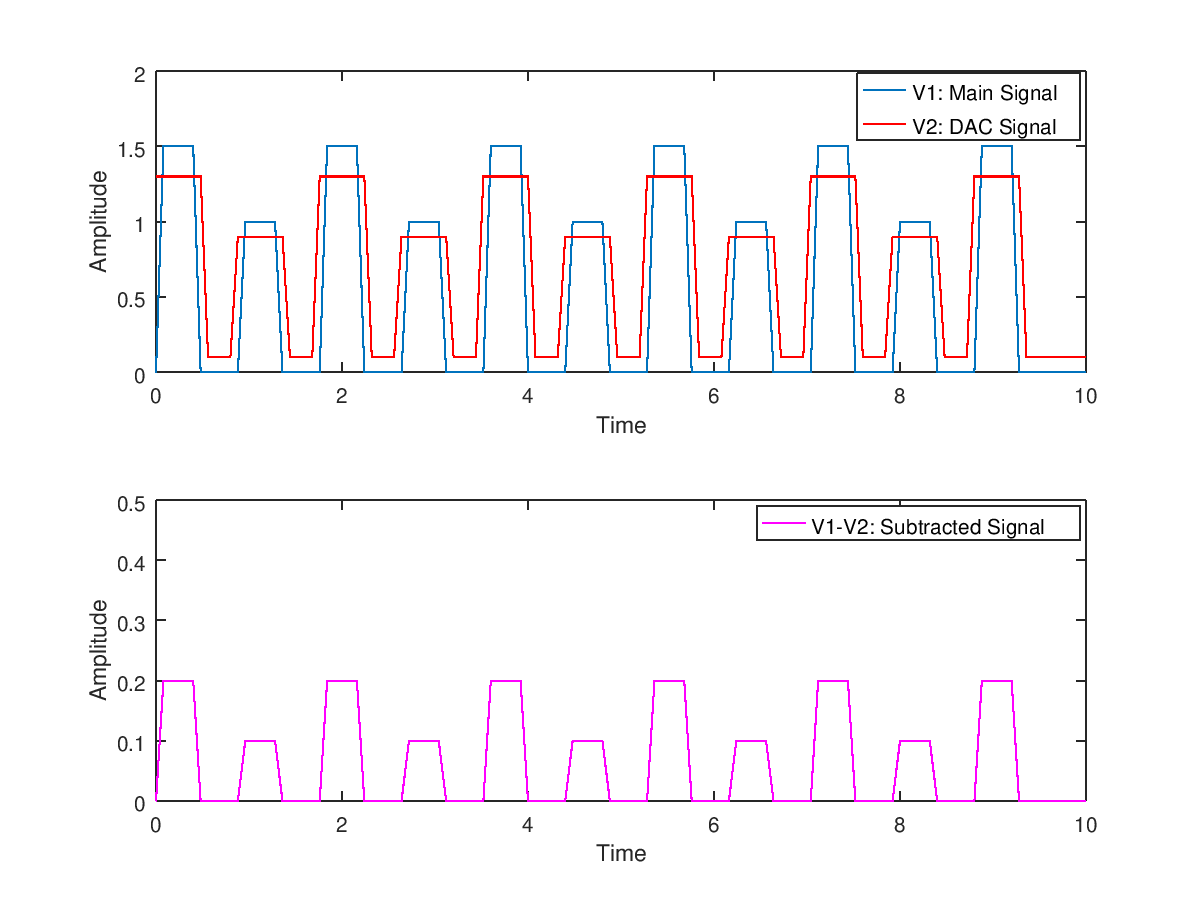
\includegraphics[width=0.8\textwidth]{../common/circuit/diff.png}
				\caption{डिफ़ैंस एम्पलीफायर का प्रभाव}
				\label{fig:diff}
			\end{figure}	
			
			यदि हम DC स्तर को पूरे सिग्नल से घटा सकें, तो केवल AC ही रहेगा जिसके स्तर को आसानी से आगे बढ़ाया जा सक़ता है। यह DC संकेत उत्पन्न करने के लिए 8 बिट डिजिटल से एनालॉग कनवर्टर (DAC) के साथ एक डिफ़ैंस एम्प्लीफायर का उपयोग यहां किया गया है। चूंकि लाल और इन्फ़्ररेड के अलग-अलग स्तर होते हैं, इसलिए DAC द्वारा स्पंदित आवृत्ति के अनुसार अलग-अलग डीसी स्तर उत्पन्न होते हैं।
			\medskip 
			
			जैसा कि चित्र \ref{fig:diff} में दिखाया गया है, Octave में उत्पन्न एक प्लॉट आवश्यक सिग्नल और डिफ़ैंस सिग्नल के घटाव को दर्शाता है। अब इस अंतर को और आगे बढ़ाया जा सक़ता है। डिफ़ैंस सिग्नल की पल्स चौड़ाई आवश्यक सिग्नल से थोड़ी बड़ी होती है ताकि आउटपुट सिग्नल में किनारों पर कोई स्पाइक न हो। डिफ़ैंस सिग्नल का निचला स्तर 0V से थोड़ा ऊपर है, जिससे अंतर हमेशा आवश्यक सिग्नल के 0V क्षेत्र में नकारात्मक हो और चूंकि ओप-अम्प एकल आपूर्ति पर परिचालन कर रहा है, इसलिए आउटपुट यहां 0V होगा।
			
			
			\begin{figure}[ht!]\centering
				\begin{circuitikz}[american] 
					\draw
					
					(4,3) node[op amp,yscale=-1] (opamp) {}
					(opamp.down) -- +(0,0.3) node[vcc]{Vcc}
					(opamp.up) -- +(0,-0.3) node[ground]{}
					(opamp.-) to [R, l^=$R_1$] ++(-2,0) node[label={left:$V_{dac1}$}] {}
					(opamp.+) to [R, l^=$R_1$] ++(-2,0) node[label={left:$V_1$}] {}
					(opamp.+) to [R, l^=$R_2$] ++(0,2) node[ground,rotate = 90]{}
					(opamp.-) -- ++(0,-1.7) -- ++(0.5,0)
					to [R, l^=$R_2$] ++(1.5,0) -- ++(0.4,0) to (opamp.out)
					(opamp.out) -- ++(1,0) to [open,v=$V_2$,o-o] ++(0,-3) node[ground]{};
			
				\end{circuitikz}
			\end{figure}
			

			\[
			V_2 = \frac{R_1}{R_1}(V_1 - V_{dac1})
			\]
			
			
			यदि, $R_1 = 10K$,
			
			\[
			V_2 \approx V_1 - V_{dac1}
			\]
		
			
		\subsubsection{प्रोग्रामेबल एम्पलीफायर}
		
			सिगनल को बढ़ाना आवश्यक हो जाता है क्योंकि त्वचा की टोन, सेंसर के साथ अनुचित उंगली संपर्क या किसी भी त्वचा रंजकता\cite{skin} से सिगनल में क्षीणन होता है। यह चरण चयन योग्य परिवर्तनीय लाभ प्रदान करता है जिसे माइक्रोकंट्रोलर द्वारा निर्धारित किया जा सक़ता है।
			
			$\mu$C निर्धारित करेगा कि किस स्तर के प्रवर्धन की आवश्यकता है और संबंधित सिगनल पिन को उच्च ड्राइव करेगा ताकि संबंधित अवरोध चयनित हो जाए।
			
			
			\begin{figure}[ht!]\centering
				\begin{circuitikz}[american] 
					\draw
						(2,3) node[op amp,yscale=-1] (opamp) {}
						(opamp.down) -- +(0,0.3) node[vcc]{Vcc}
						(opamp.up) -- +(0,-0.3) node[ground]{}
						(opamp.+) to ++(-2,0) node[label={left:$V_2$}] {}
						(opamp.-) -- ++(0,-1.7) -- ++(1,0)
						to [R, l^=$10K$] ++(1,0) -- ++(1,0) -- ++(0,2.2) to (opamp.out)
						(opamp.-) ++(0,-1.7) -- ++(0,-1.5) to [R, l^=$10K$] ++(0,-1) -- ++(0,-0.5)
						++(0,-0.5) node[npn] (Q1){}
						(Q1.E) node[ground]{}
						(Q1.B) to [R, l^=$4.7K$] ++(-1.5,0) node[label={left:S1}] {}
						
						(opamp.-) ++(0,-1.7) ++(0,-0.75) -- ++(3.5,0) -- ++(0,-0.75)		
						to [R, l^=$4.7K$] ++(0,-1) -- ++(0,-0.5)
						++(0,-0.5) node[npn] (Q2){}	
						(Q2.E) node[ground]{}	
						(Q2.B) to [R, l^=$4.7K$] ++(-1.5,0) node[label={left:S2}] {}
						
						(opamp.-) ++(0,-1.7) ++(0,-0.75) ++(2,0) -- ++(5,0) -- ++(0,-0.75)		
						to [R, l^=$2.35K$] ++(0,-1) -- ++(0,-0.5)
						++(0,-0.5) node[npn] (Q3){}	
						(Q3.E) node[ground]{}	
						(Q3.B) to [R, l^=$4.7K$] ++(-1.5,0) node[label={left:S3}] {};
						
						
				 \end{circuitikz}
			\end{figure}	
	
			\begin{center}
				\begin{tabular}{ |c|c|} 
					\hline
					\textbf{स्विच} & \textbf{बढ़त}   \\ 
					\hline
					सभी बंद & 1 	 \\ 
					\hline
					S1 & 2  		\\ 
					\hline
					S2 & 3  		\\ 
					\hline
					S1+S2 & 4  		\\ 
					\hline
					S3 & 5  		\\ 
					\hline
					S1+S3 & 6	  	\\ 
					\hline
					S2+S3 & 7  		\\ 
					\hline
				\end{tabular}
			\end{center}
	
	
	\subsection{LED चालक}

	
		जैसा कि पहले चर्चा की गई थी, ट्रांस्इम्पेडेंस चरण के बाद सिगनल स्तर बहुत कम हो सकता है। led ड्राइवर को आवश्यकतानुसार led के केरंट बढ़ाना की जरूरत है। निम्नलिखित सर्किट का उपयोग वोल्टेज नियंत्रित करंट स्रोत के रूप में किया गया है, वोल्टेज को DAC सेट करता है $\mu$C के निर्देशन पे।
		
		\begin{figure}[ht!]\centering
			\begin{circuitikz}[american] 
				\draw
				
				(4,3) node[npn] (Q1){}
				(Q1.E) to [R, l^=20] ++(0,-1.5) node[ground]{}
				(Q1.B) to [R, l^=4.7K] ++(-1.5,0) node[label={left:$V_{dac2}$}] {}
				(Q1.C) -- ++(-1,0) -- ++(0,0.5) ++(0,0.5)  node[npn] (Q2){}
				(Q2.B) to [R, l_=10K] ++(-1.5,0) node[label={left:Red pulse}] {}
				(Q2.C) -- ++(0,1) node[]{} ++(0,0.2) node[]{Red cathode}
				(Q1.C) -- ++(1,0) -- ++(0,0.5) ++(0,0.5) node[npn,xscale=-1] (Q3){}
				(Q3.B) to [R, l^=10K] ++(1.5,0) node[label={right:IR pulse}] {}
				(Q3.C) to ++(0,1) node[]{} ++(0,0.2) node[]{Ir cathode};
			\end{circuitikz}
		\end{figure}
		
		
		जब भी लाल/इन्फ्रारेड पल्स सक्रिय होता है, तो led एकल पुल विन्यास द्वारा सक्रिय हो जाते हैं, संबंधित लाल/इन्फ्रारेड led सक्रिय हो जाते हैं (Vcc से जुड़े led एनोड)। करंट की मात्रा $V_{dac2}$ \& $R_1$ पर निर्भर करेगी।
		
		$V_{dac2}$ भी स्पंदित आवृत्ति के अनुसार लाल और इन्फ़्रारेड के लिए अलग-अलग सेट किया जायेगा। यदि सिग्नल का पता लगाने के लिए तीव्रता पर्याप्त नहीं हो, तो $V_{dac2}$ को बढ़ाना आवश्यक है। $\mu$C थ्रेसहोल्ड का निर्धारण करेगा और उसके अनुसार नियंत्रण वोल्टेज को संशोधित करेगा।	

		प्रोग्रामेबल एम्पलीफायर चरण के बाद अंतिम आउटपुट नीचे दिखाया गया है। प्राप्त PPG सिग्नल - लाल और इन्फ़्ररा-रेड स्पष्ट रूप से दिखाई दे रहे है और एक उपयुक्त स्तर पर है जिसे ADC को भेजा जा सक़ता है ऐल्गोरिद्म मे उपयोग के लिये। 
	
	\begin{figure}[ht!]
		\centering
		\subfloat[अंतिम आउटपुट - हरा, V\textsubscript{1} - नीला
		]{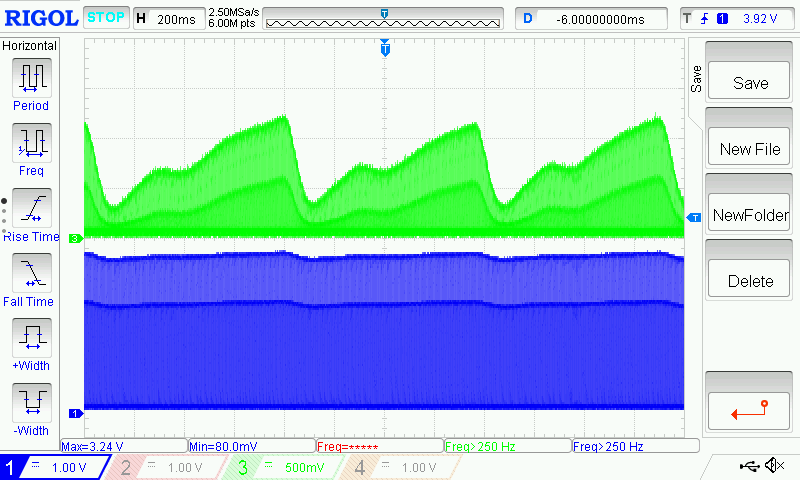
\includegraphics[width=1\textwidth]{../common/circuit/final_out.png}}
		\hfill
		\subfloat[अंतिम आउटपुट का माप
		]{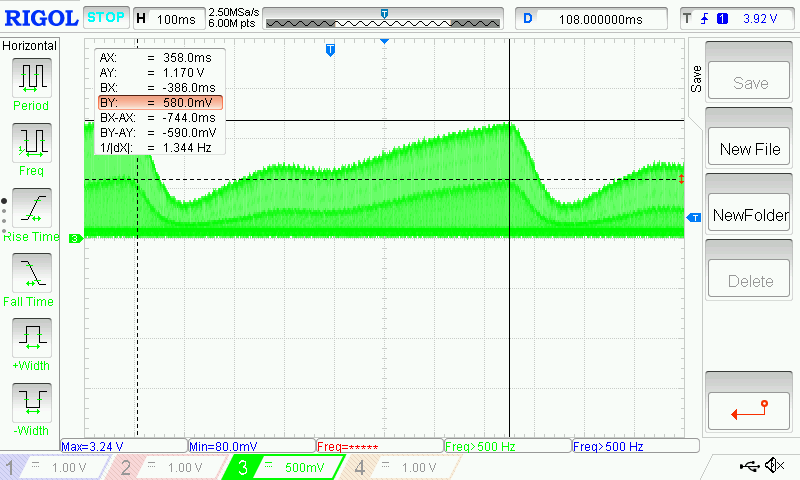
\includegraphics[width=1\textwidth]{../common/circuit/final_out_meas.png}}
		\caption{अंतिम आउटपुट}
	\end{figure}	
	